\documentclass[tikz,border=2pt]{standalone}
\usepackage[T1]{fontenc}
\usepackage{lmodern}
\usetikzlibrary{arrows.meta,decorations.pathreplacing}
\begin{document}
\sffamily
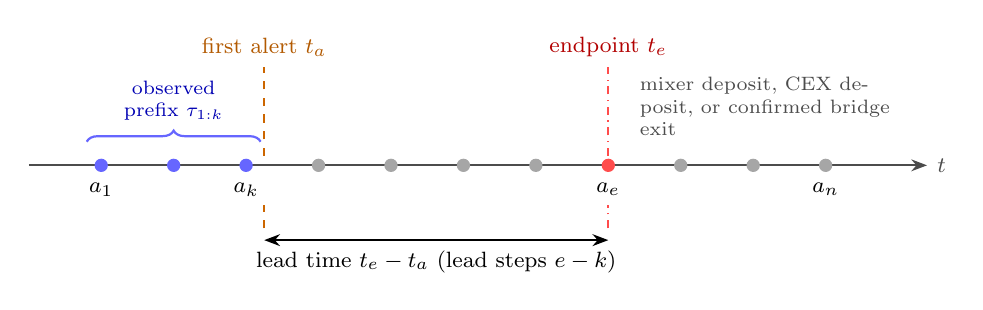
\begin{tikzpicture}[font=\footnotesize, x=0.92cm]
\draw[-{Stealth[length=2mm]}, thick, black!70] (0,0) -- (12.4,0) node[right] {$t$};
% actions
\foreach \i/\c in {1/blue!60,2/blue!60,3/blue!60,4/black!35,5/black!35,6/black!35,7/black!35,8/red!70,9/black!35,10/black!35,11/black!35} {
  \fill[\c] (\i,0) circle (2.4pt);
}
\node[below=3pt] at (1,0) {$a_1$};
\node[below=3pt] at (3,0) {$a_k$};
\node[below=3pt] at (8,0) {$a_e$};
\node[below=3pt] at (11,0) {$a_n$};
% prefix brace
\draw[decorate, decoration={brace, amplitude=4pt}, thick, blue!60] (0.8,0.3) -- (3.2,0.3) node[midway, above=4pt, blue!70!black, align=center, font=\scriptsize] {observed\\prefix $\tau_{1:k}$};
% alert and endpoint
\draw[dashed, thick, orange!80!black] (3.25,-0.8) -- (3.25,-0.5); \draw[dashed, thick, orange!80!black] (3.25,0.12) -- (3.25,1.25) node[above, orange!70!black] {first alert $t_a$};
\draw[dashdotted, thick, red!70] (8,-0.8) -- (8,-0.5); \draw[dashdotted, thick, red!70] (8,0.12) -- (8,1.25) node[above, red!70!black] {endpoint $t_e$};
% lead time
\draw[{Stealth[length=2mm]}-{Stealth[length=2mm]}, thick] (3.25,-0.95) -- (8,-0.95) node[midway, below] {lead time $t_e-t_a$ (lead steps $e-k$)};
\node[anchor=west, text width=3.3cm, align=left, font=\scriptsize, black!70] at (8.3,0.75) {mixer deposit, CEX deposit, or confirmed bridge exit};
\end{tikzpicture}
\end{document}
